\chapter{Implementation}
\label{Implementation}
	The implementation phase of the software design consists of different tasks to be done sequentially for obtaining the desired results. There are two modules: user module and background module. The different phases are:
\begin{itemize}
\item Creating Graphical User Interface: GUI is created in eclipse under Android SDK 4.0 for a user friendly interface. It is intended for two purposes. First is to create a user friendly interface for the software. Having a good user interface makes it easier for the user to use and understand the different functionalities of the software. Secondly the user interface hides the end users from the complexities in the working of the software.

\item Creating System Environment: For the intended project to work on, it need to implement hardware and software requirements. This system is build using visual studio 2010 under .NET framework and Android platform using eclipse based on Windows operating system.

\section{Screen shots}
\label{Screen shots}
In this chapter,the screen shots of the results achieved in different stages had been displayed. The screen shots of launcher and terms and conditions are shown below. Here launcher(fig 5.1), the progress bar used to shows the loading of application. Terms and conditions(fig 5.2), shows academic project development license and a new user must accept this license.
\newline 	Other screen shots such as user registration, user login, connection window, system configuration, home options, remote desktop access, send notification, power options and message notification has shown in appendix.
\newline User registration window shows mobile user can register by providing his/her username and password. User Login, registered users can login with username and password. Connection window contain two options: connect to PC and Create Network. When create network option selected control goes to the settings of android. System configuration connect the PC to android through IP address. Home option have four selection options: desktop mode, send notification, power options and disconnect. The remote desktop shows the desktop of PC in android touch screen. Send notification used to send message to the remote child PC. Power option contains, shutdown, hibernate, restart, lock, logoff and sleep. Message notification shows the message from android.  
	
\begin{figure}
\subsection{User Interfaces}
\label{User Interfaces}
\begin{center}
\scalebox{0.25}
%{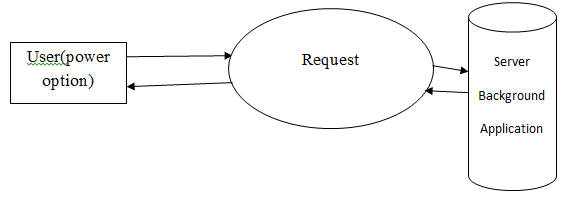
\includegraphics{power1.png}}
{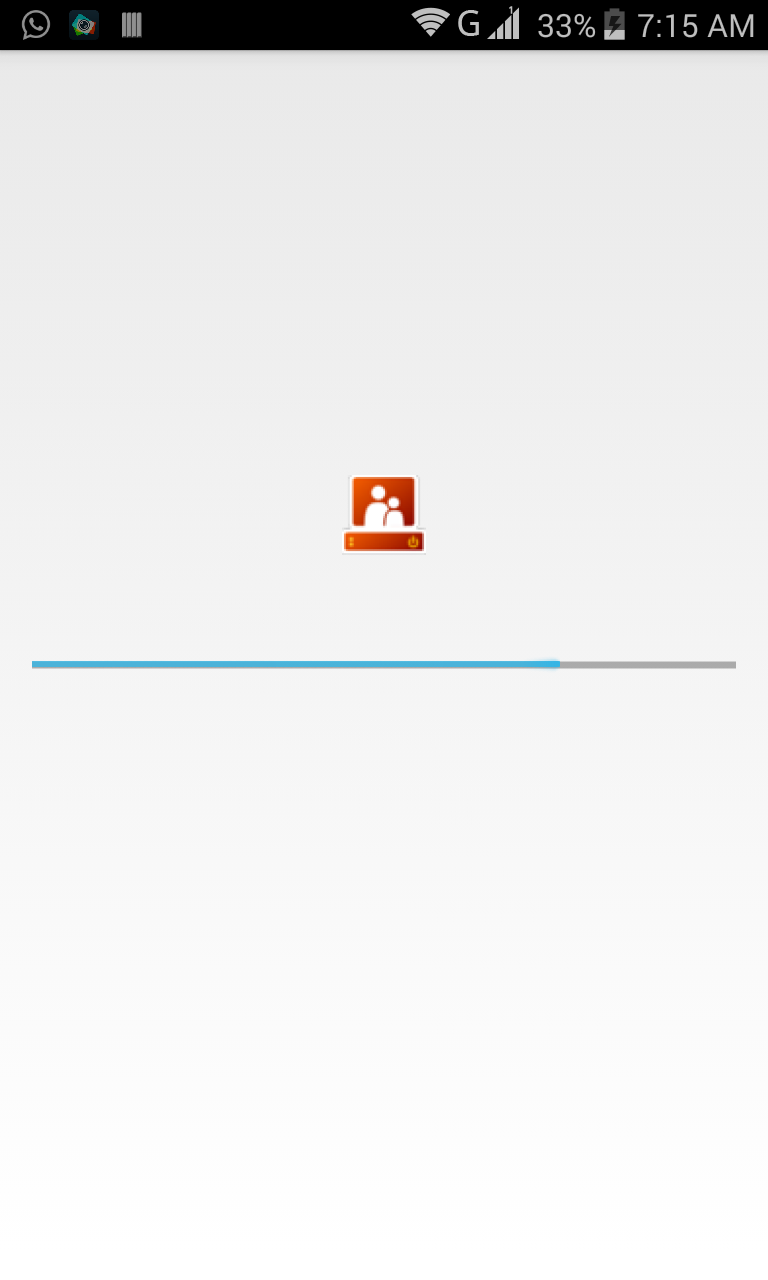
\includegraphics{launch.png}}
\caption{Launcher}  
\end{center}
This window shows loading of application.
\end{figure}


\begin{figure}
\begin{center}
\scalebox{0.25}
%{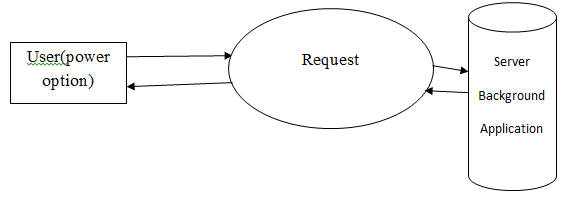
\includegraphics{power1.png}}
{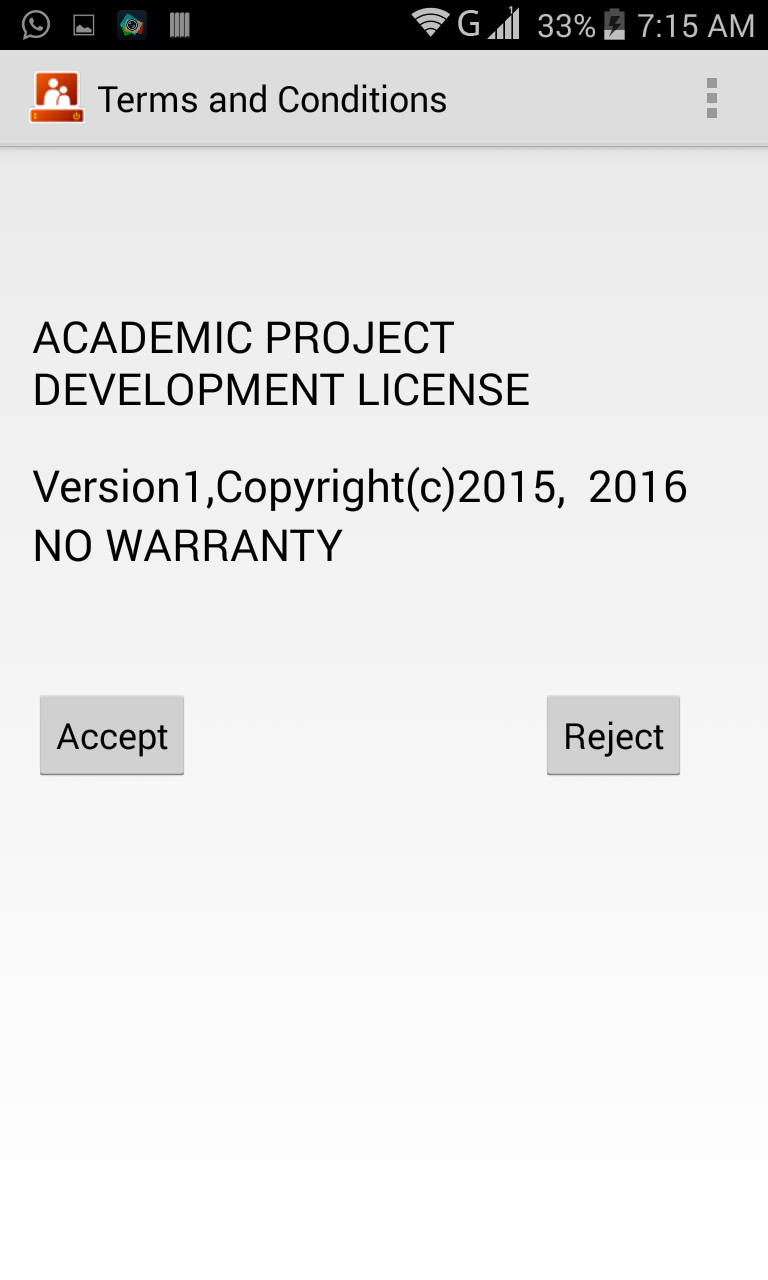
\includegraphics{terms.png}}
\caption{Terms and Conditions}  
\end{center}
This window shows academic project development license.
\end{figure}